\documentclass[a4paper]{article}
\usepackage{lipsum}
\usepackage{url}
\usepackage{graphicx}
\usepackage{listings}
\lstset{language=Python}
\usepackage[margin=2cm]{geometry}
\graphicspath{ {images/} }

%Custom Commands
\newcommand{\Pokemon}{Pok\'{e}mon}
\newcommand{\Pokeapi}{Pok\'{e}api}

\begin{document}

\begin{titlepage}
	\newcommand{\HRule}{\rule{\linewidth}{0.5mm}}
	\center{}

    %Headings
	\LARGE{University of Nottingham}\\[1.5cm]
	\Large{Computer Science with Artificial Intelligence MSci}\\[0.5cm]
	\large{G53IDS - Individual Dissertation}\\[0.5cm]

    %Title
	\HRule{}\\[0.4cm]
	{\huge\bfseries Applying Evolutionary Algorithms to \Pokemon{} Team Building}\\[0.4cm]
	\HRule{}\\[1.5cm]

    %Authors
	\begin{minipage}{0.4\textwidth}
		\begin{flushleft}
			\large
			\textit{Author}\\
			Benjamin \textsc{Charlton}\\
            psybc3@nottingham.ac.uk\\
            4262648
		\end{flushleft}
	\end{minipage}
    \begin{minipage}{0.4\textwidth}
		\begin{flushright}
			\large
			\textit{Supervisor}\\
			Prof.\@ Bob \textsc{John}\\
            Robert.John@nottingham.ac.uk
		\end{flushright}
	\end{minipage}

    %Date
	\vfill\vfill\vfill
	{\large24\textsuperscript{th} April 2018} %TODO WHAT DATE
	\vfill

\end{titlepage}

%Contents Page
\tableofcontents
\pagebreak

%TODO WORK OUT ALL OF THE SECTIONS
\section{Introduction}
\subsection{Introduction}
\par
Video games are an ever growing field of interest for many people.
Like many games people play competitively against each other and in some cases their are tournaments on an international scale with whole teams set up to win the large prize pools\cite{eSportsPrize}\cite{teamEarnings}.
This field has become to be known as eSports.
\par
Game playing is an obvious application of AI techniques as you can objectively score wins and losses.
Initially this has been seen with traditional board games like Chess\cite{deepBlue} and Go\cite{alphaGo}.
During The International 2017 for DotA 2 this all changed as the worlds of AI and eSports came together in a 1v1 show match\cite{openAI}.
Elon Musk, backer of this initiative, said that this is `Vastly more complex than traditional board games like chess \& Go'\cite{openAI}.
Typically in these set ups their is no decisions to be made prior to the game itself, in fact to limit the DotA 2 AI they limited it to a preselected character to play with.
\par
Many strategy games have a decision making element before the game is played.
Collectable Card Games (CCGs) have the choice of which cards to put in your limited deck or in \Pokemon{} you have to choose which members of your team to use and how you have trained them.
This element of the games is refereed to as deck/team building as the player has to build up what they bring to the game from an empty deck or team.
Some players are very good at playing the game but not very good at choosing which deck/team to bring resulting in a practice called `netdecking', being called so as the player will take someone else's deck/team from the internet instead of coming up with their own.
\par
\Pokemon{} has a tricky team building process that is rather hard for new players to comprehend.
In the build up to the annual \Pokemon{} World Championships, many players will go through the tedious process of team building to make sure they have the right strategies and counters in place to bring to the matches ahead\cite{worldsOverview}.
This requires expert knowledge such as type match ups and speed tiers along side several rules of thumb.
Once a general strategy is in place the players must perform several calculations to optimise the statistics of their team, optimising offensive stats to faint certain threats or optimising defensive stats to allow the team to survive after certain moves are used against them.
\subsection{Motivation}
\par
The motivation for this project comes partly from the novelty of the idea.
As evolutionary algorithms are designed to simulate survival of the fittest could it work on a representation of a biological population.
In the \Pokemon{} games there is an idea that their is a living ecosystem with predators and prey as well as a system for the \Pokemon{} to fight in combat to decided who is the strongest.
\par
Further motivation comes from the seeing how AI game playing is progressing and trying to create something that will combat other aspects that come into playing video games.
This approach could be useful for players of the game allowing them to find new and winning strategies that might not have previously been known.
It could also help the development team behind the games balance the game despite the ever increasing mass of combinations that they have to consider.
\subsection{Aims and Objectives}
\par
This project aims to implement a evolutionary algorithm that will create a \Pokemon{} team.
The output of such will be a team of \Pokemon{}, including all of the vital statistics and moves; this would be dependant of the format.
These results will be then compared to human designed solutions to conclude if the evolutionary algorithm is comparable to an expert.
\\ \\The objectives of this project are:
\begin{enumerate}
    \item Research evolutionary algorithm methods used to approach similar problems.
    Looking in detail about issues such as representation, evaluation and validity of the chromosomes.
    This information will be used to help direct how best to approach the problem and design the system.
    \item Design an effective and efficient way to model and represent the problem in the evolutionary algorithm while still maintaining relevant data to the problem.
    This will also be used to form the output so will need to be readily be able to translate into a readable format for the user to understand.
    \item Develop a Genetic and Memetic algorithm to tackle the problem from scratch, including conventional and unique methods for the various stages in the algorithms.
    Making sure that all of the elements of the code base are created in a fashion that allows for reusability and adaptation.
    For example both the Genetic and Memetic algorithm could share the methods like objective evaluation and selection.
    This will all be developed from scratch (bar the use of a few relevant APIs).
    \item Compare and analyse the results of each evolutionary algorithm (with a variety of settings) with each other and human designed solutions.
    Solutions for comparison will come from readily available teams from top players and analysis will be taken by evaluating the solutions.
    If solutions are viable enough they can be input into the game and used in some real world settings such as battling with other players, rather than being graded by a score.
\end{enumerate}

\section{Related Work}
%\begin{itemize}
%    \item Investigate more works to talk about here (gaming and more general)
%    \item GAs, MAs and other EAs
%\end{itemize}
\subsection{AI and Game Playing}
Many AI approaches to games tackle the aspect of playing the matches and the decision making process to choose the best action.
Lots of research and development has happened in these areas with many effective techniques being discovered.
One key reason the problem of prematch decision making hasn't been tackled is due to the lack of need for it with classical table top games requiring no preparation before the match begins.
\\ \par
Chess was an early and significant example in the history of AI, with the Deep Blue computer from IBM successfully beat the at the time world champion Garry Kasparov\cite{deepBlue}.
This was significant as creating a winning chess AI was seen to be the next big milestone at the time in AI\@.
To achieve this Deep Blue used a combination of techniques with the main underlying AI technique being a search method.
To achieve this at the time custom hardware was created to help speed up the computation with a highly parallel structure that could evaluate nodes on the search tree quickly using hardware implementations.
This meant that it could effectively search deeper than any other AI at the time.
\par
Go is the most recent milestone game to be beaten with AlphaGo claiming its victory against one of the best Go players, Lee Sedol, in March 2016\cite{alphaGo}.
To achieve this the team uses Deep Neural Networks combined with Monte Carlo tree search, with a combination of supervised learning from human games and reinforcement learning via self-play.
\par
Recently AlphaGo has been beaten by a variation of itself AlphaGoZero, named as it had learnt from zero human knowledge\cite{alphaGoZero}.
AlphaGoZero learnt entirely from self-play and achieved super human performance.
This shows that not only can AI techniques successfully solve tasks but it is possible to do so with no expert knowledge.
\\ \par
As the field of AI game playing moves forward into more complex games prematch decisions will need to be considered.
With current methods it would be rather simple to build and train an AI to play turn based strategy games, such as collectable card games or in this case \Pokemon{}, but the deck/team building would require an expert to decide what the AI will be trained to use.
This is often problematic as season rotation could add in new elements to the game or make certain elements no longer useable, or shifts in the metagame will mean that the AI is easily countered.
\par
Team building is a form of optimisation problem as you are trying to bring the optimal team to the match so you have the best chance of winning.
\par
A variety of work has been conducted looking at optimisation via AI techniques, in this review of previous works a focus has been upon techniques that tackled having a large, vast search space and where the correctness of a solution was hard to judge.
Both of these issues are problems that will have to be over come in building this project.
\subsection{Hearthstone Deck Building GA}
\par
Garc{\'\i}a-S{\'a}nchez et al.\ tackled a very similar problem using a genetic algorithm to approach deck building\cite{hearthstoneAI}.
The example they used was a popular collectable card game, Hearthstone, and they tried to create a viable competitive deck through the genetic algorithm.
This is of particular interest as several parts of their study directly relate to what the project is trying to achieve, as well as several short comings that will have to take into account.
\par
An evolutionary algorithm was used as `they commonly produce very effective combinations of elements'\cite{hearthstoneAI}, which a deck can be described as a combination of cards.
This also allowed for competitive decks to be built from scratch with no expert knowledge required.
This was done by encoding the individuals as a vector of cards, in this case the 30 element vector became the deck.
\par
In the deck building process it was possible to have a deck that would violate the rules of the game.
To discourage the EA from creating decks that violate these rules; a correctness metric was taking into account when calculating the fitness of each individual.
If an individual was incorrect it wasn't evaluated further in the fitness calculation process and given the worse possible score\cite{hearthstoneAI}.
\\ \par
A large part of the work talks about the fitness evaluation, as with many of these processes it is hard to quantify how well a individual will do.
Even though human experts will have a strong intrinsic idea to what is better or worse, they will often playtest their ideas for several matches, sometimes ranging into the hundreds, before applying some analysis to develop their idea further.
To give the most realistic simulation a separate AI played each individual against some previously expert designed decks, that have been proven to be successful in the metagame that the AI was evolving in.
It played several matches with each individual against the decks, with 16 matches versus the 8 chosen opponent decks totalling 128 matches per individual\cite{hearthstoneAI}.
\par
One of the key upsides of this was that the GA could evolve to combat common decks that it would face if it was to be played in competitive play.
Knowledge of key opposing threats is something that high level experts take into account, this knowledge was taken from an article evaluating the current meta game written by professional players of the game.
Another upside was from having a high number of matches being played for the evaluation; by playing a large proportion of games they can mitigate any randomness in the matches that aren't down to the deck building, such as the cards in the starting hand.
To further mitigate randomness and to give a more accurate representation of the individuals fitness, statistical analysis was used to calculate the final fitness score.
This was done to also as it is important to find `a deck with a fair chance to win against all decks in the metagame' not one that is strong against a particular opponent and weak to all others.
\par
Through this method of fitness evaluation some flaws and potential shortcomings where brought up.
As the fitness evaluation required a large amount of matches to be played it resulted in `every execution of the algorithm requires several days'\cite{hearthstoneAI}, even when running on a small population size and number of generations (10 and 50 respectively).
Although not a specifically a bad thing a longer run time would discourage the use of such tools, more so in games where the meta game changes more rapidly.
The evaluation also required the expert knowledge of the meta decks to be tested against or even that an established meta is in effect where as many experts can theory craft a rough idea before changes to the meta happen.
The most significant flaw with this style of evaluation is that it relies on the ability of another AI to pilot the deck.
It was suggested that it may overfit `with regards to the AI capabilities and playing style' even going as far as pointing out that it `can use some decks (and some playing styles) better than others'\cite{hearthstoneAI}.
\subsection{Genetic Algorithms}
\par
Maumita Bhattacharya spoke about differing approaches to the problem of computationally expensive fitness evaluation\cite{expensiveOptimisation}.
Several of the techniques described approximated the fitness of each individual while only periodically calculating a more accurate value.
Some of these techniques achieved this my simulating a simpler model while more specific techniques where discussed too.
In a population search method like evolutionary algorithms, a technique called Fitness Inheritance could be used.
As the children individuals will closely resemble the parents you could give a rough approximation to how different they actually are and use that difference to evaluate the children.
This will greatly reduce the number of computationally expensive evaluations you need to do with potentially as few as only scoring the initial population.
However it is suggested that you periodically recalculate using the true fitness evaluation as `Using true fitness evaluation along with approximation is thus extremely important to achieve reliable performance'.
\par
Fitness Inheritance was first proposed by Smith et al.\cite{fitnessInheritance} where they applied the idea to a simple problem OneMax.
They investigated two simple methods to inherit fitness.
Averaged Inheritance simply said `a child is assigned the average fitness of its parents', this is extremely cheap computationally and requires no detailed analysis.
Another method was Proportional Inheritance where `the average is weighted based on the amount of genetic material taken from each parent', while slightly more expensive it takes into account of none symmetric crossover schemes such as one point crossover where the genetic material is not equal from each parent.

\section{Methodology}
%\begin{itemize}
    %\item Citations
%\end{itemize}
\subsection{Evolutionary Algorithms}
%\begin{itemize}
%    \item Choice of GA and MA
%    \item Why this over other AI techniques like ANN and Local Search
%\end{itemize}
\par
The main AI technique behind this project is evolutionary algorithms, this technique has been chosen as it successful optimises problems with little expert knowledge as shown in the related works.
There are a few different types of evolutionary algorithms, with genetic algorithms and memetic algorithms being focused on in this project.
The reasoning for choosing these two types is that they are closely related and will allow for a lot of the code to be shared between them, in fact a memetic algorithm can be seen as an extension of a genetic algorithm.
Another potential extension would be a multimeme memetic algorithm but the scope of the project does not allow time to develop this.
\par
The key advantage of evolutionary algorithms is that they can effectively explore the search landscape due to their population based search method, a critical feature in this problem as there are a a lot of possible combinations to search through.
For example in a team of \Pokemon{} each team member on a team of 6 can be chosen from the 805 different species of \Pokemon{}.
This gives the following number of possibilities:
\begin{equation}
{species \choose teamSize} = {807 \choose 6} = 3.765 \times 10^{14}\ (4sf) %376,545,899,656,927 to be exact
\end{equation}
\par
Once you begin to factor the the other potential values it becomes a lot larger very quickly, a rough estimate for the number of possibilities is as follows:
\begin{equation}
{species \times IVs^{stats} \times EVs^{stats} \times levels \times happiness \times abilities \times genders \times items \times {moves \choose move slots} \choose teamSize}
\end{equation}
\begin{equation}
    {807 \times 31^6 \times 256^6 \times 100 \times 256 \times 3 \times 2 \times 354 \times {728 \choose 4} \choose 6} = 5.893 \times 10^{261}\ (4sf)
\end{equation} % 5892646138241710986407793497445852707778105080508958016801817373764061910688657477422986377898950796546392632127158482762259927547606249722743913164896701603448604234412592111287339200538369501817891667466913812521600691151442407389407976543054201078289530880000 exactly :P
\par
Although this is an astronomically large search space, a large proportion of these possibilities will be invalid solutions as if any of the team members aren't valid then the whole solution becomes invalid.
By using a evolutionary algorithm this search space can be quickly explored and iterated upon.
\par
Another advantages of evolutionary algorithms is that they allow for the usage of both domain specific methods and more general methods, potential to be parallelised, ability to translate the solution to a human understandable result and the simplicity of the overall concept.
\\ \par
The issues with these techniques come from how to accurately represent the problem in a form that can be easily manipulated by the algorithm.
This is rather complex on real world problems and requires careful thought and design to mitigate any issues later down the line.
Another issue comes from need to score each solution, in this problem there is no real objective way to score a solution.
Practically an EA also has the issue of run time, like most AI techniques they are very computationally expensive and having a longer run time will result in more optimal answers.
\\ \par
Evolutionary algorithms were chosen over other AI techniques not only due to the advantages above but as there are issues with other techniques when approaching this problem.
\par
As shown with the calculations above, brute force methods are unfeasible as the search space is far too large.
Even if you effectively limited the search space by employing several powerful domain specific heuristics or pruning of the search space it would not limit it enough to allow for brute force methodologies.
Brute force methods still suffer from the lack of an objective score for each solution to be able to return the best result.
\par
Many techniques such as Decision Trees and Support Vector Machines concentrate on classifying the result based upon an already labeled dataset that they learned form.
To adapt the problem into a classification style problem would be impractical as mentioned earlier it would be hard even for human experts to say what is good and bad to classify a solution.
Artificial Neural Networks also approach classification problems effectively and thus have similar issues to other classification problems
Although human made solutions exist there is not a mass of solutions to learn from so these machine learning techniques aren't easily applicable.
\par
Mathematical optimisation techniques can't be effectively used to calculate an optimum as the objective value that you are trying to optimise is extremely difficult to calculate.
Other AI optimisation techniques could be used to solve this problem, such as Local Search methods.
The key draw back of the local search methods is defining a move operators for this problem, as it is such a high dimensionality problem and not all of the dimensions have obvious move operators.

\subsection{Object Orientated Design and Python}
%\begin{itemize}
%    \item Easy adaptation
%    \item Conversation from GA to MA
%    \item Commonly used, lots of APIs
%\end{itemize}
The project will be coded in Python, a powerful Object Orientated programming language.
Python was chosen due to its strong object orientated design features that will be rather suitable for coding of evolutionary algorithms.
By following several object orientated design practices the project will be easily adaptable through out development, primarily allowing for the easy adaptation to the MA further in the project by reusing multiple classes.
\par
Python was also chosen as it is a very commonly used language, being the 3\textsuperscript{rd} most popular language on GitHub\cite{GitHut} as of the writing of this report.
This popularity means that there is extensive resources on the language and it goes to show how powerful it is.
Alongside its popularity comes many usable APIs, although the project is going to be mainly created from scratch at some points the use of an API might be relevant, and it should be simple to find one that will suit the needs of the project.

\subsection{Software Engineering Tools}
%\begin{itemize}
    %\item Git
    %\item Latex
    %\item Atom
    %\item How these tools work together and help with project management and speed up work
    %\item Citations to show that these are good tools
%\end{itemize}
\par
To aid with the large scope of this project, a variety of software engineering tools are being used.
This section will list some of the larger tools and processes that they provide.
\subparagraph{Git}
Git is a version control system the main draw of such a technology is to allow for easy restoring of code to a working state if a change breaks something.
This is done by having a tree of `commits' within each are the changes to the files at that point, normally stored as line differences in the code files; at any point you can go back in the tree to a commit that needs to be reverted too.
The tree structure can also branch to allow different modifications to be made, this feature is currently being used to allow for documentation and code to be written at the same time.
It will useful later on with the adaptation from the GA to the MA, allowing a stable branch with working GA code in it and a MA branch that is modifying the same files.
\par
To use the Git system there are a few pieces of software being used.
Although you can work on a local repository, it is highly recommended that a remote repository is used as a form of backup and allows for the code base to be worked upon from multiple devices so long as the remote repository is up to date.
The project will be stored on the School of Computer Science GitLab server, leveraging the functionality of the remote repository while keeping the project private for the foreseeable future.
\subparagraph{LaTeX}
LaTeX is a software to help with documentation preparation, which has been used to create all of the documents thus far.
A key reason to use this is that it stores the source files in a manner that allows for Git to effectively show the changes.
This allows for the entirety of the project to leverage the Git repository rather just the code base.
\par
Referencing is a lot easier in LaTeX as during the compile it will automatically work out what the correct references are with easily human readable tags for each citation.
Another feature of LaTeX is the use of images, by storing them in a separate folder and loading them in any changes that I make to the image will be replicated in the document.
Although it has taken some time to get used to the nuances of LaTeX it is allowing for much more powerful and granular control of the documentation writing, while relieving stresses such as how parts are brought together.
\subparagraph{Atom}
Both the code and the documentation are being written in a text editor called Atom.
The main use of Atom in this project is that it edit both the code and documentation simply by installing packages to recognise both languages.
Additional packages have also been installed to allow for easy compilation and viewing of the LaTeX files and a project management system which will save the workspace for the various segments of the project.
It also integrates well with Git showing which files and specific lines have been modified, allowing for easy management at a glance.
\\ \par
Together all of these tools help with the software engineering process by both encouraging good practice and streamlining some more complex processes.
In the long term this will help with the project management of the project by helping keeping it organised and clear.

\section{Design and Implementation}
%\begin{itemize}
%    \item Separation of settings
%    \item High level Representation Explanation
%    \item Low level Representation Explanation
%    \item Use of the benchmark example
%\end{itemize}
\subsection{Representation}
\par
Currently the representation is not fully developed but it has a general outline and some design choices that will be outlined here.
The representation is going to be a set of 6 \Pokemon{} in the team with each \Pokemon{} having its own set of variables that are required to accurately describe it for competitive play.
To allow ease of storage and compatibility with \Pokeapi{} some values will be stored as an id number that corresponds with the relevant data in the API\@.
Other values will be stored as simple integer values or enumerations as required.
\par
This representation will then be presented to the user in a format known to the community as `Showdown Format' as it will be useable with the import feature of an online simulator called \Pokemon{} Showdown\cite{showdown}.
\subsection{Genetic Algorithm}
\par
The main core of the GA has been created outlining the key stages in the algorithm and setting a structure for the methods to be called upon.
To show that it is functioning correctly a simple benchmark function has been created with some simple methods to go alongside it.
\par
Some of the key design decisions have been started with this main core of the program, one such decision is the separation of hyper parameters into a settings file to allow for easy access and tuning.
Another design decision that has impacted upon the implementation is how the problems are accessed.
Each individual is represented by its own class, this allows for you to instantiate objects of that class as each member of the population.
Methods for accessing the variables and printing are also contained in this class to bring it in line with python design practices.
This will be developed further to give getter and setter methods to avoid invalid access to variables in the future.
\par
The problem is defined as its own class with all the relevant methods for the stages of the GA contained within it.
Doing so gives the main core a more simplistic design and gives the ability to have problem specific methods.
This can be developed further by having some general GA methods such as selection criteria to be defined in a separate general file and imported into the problem.

\section{Progress}
%\begin{itemize}
%    \item Current achievements in the project
%    \item Personal Reflections
%\end{itemize}
\subsection{Current Achievements}
\par
Currently the project has some code written for it, with the major achievement being the general GA structure being written in an adaptable manner, with it working on a benchmark function successfully.
There is also a basic outline of the representation being worked upon that will with further developments to come.
\par
The code for the general GA structure can be seen in the appendix, and the best solution and objective value for running the benchmark function can be seen in the table.
The benchmark function is the Sum of Squares, in this the objective value is the sum of the squares of all the elements (2 in this example) where each element can be in the range -5 to 5, as real values.
The objective function can be calculated using the following equation:
\begin{equation}
    where\ n = 2\quad \sum_{i=1}^{n} x_i^2 = x_1^2 + x_2^2
\end{equation}
This objective value is to be minimised giving a global maximum of every element being 0.
In this case the following hyper parameters were used:
\begin{equation}
    generations = 50,\ populationSize = 10,\ mutationRate = 0.1
\end{equation}
Running it 5 times gave the following results to 3 significant figures:
\begin{center}
    \begin{tabular}{ c c | c }
        x\textsubscript{1} & x\textsubscript{2} & Objective Value \\
        \hline
        0 & 0 & 0 \\
        0.866 & 0.240 & 0.807 \\
        -0.014 & -0.126 & 0.016 \\
        0.107 & 0.694 & 0.493 \\
        0.000 & -0.011 & 0.000 \\
    \end{tabular}
\end{center}
\par
Although it the reason of this simplistic benchmark function was not to test the capabilities of the GA or any of the methods created it does show that the overall structure works and it can now be easily adapted to the problem with confidence that it is all working.

\subsection{Reflections on Work Plan}
\par
Through out project management has been a key consideration, both to allow clear progress to be seen and to get updates on how to move forward.
To aid with the management of the project, tasks have been reconsidered to make progress easier or to give time to tackle arising problems.
To both show and predict progress a work plan was created and has been updated to add in new tasks or extend others.
\\ \par
To aid with project management and accountability frequent meetings have taken place.
These have often discussed upcoming tasks in relation to the work plan and what work has taken place.
For each meeting a short set of minutes was created and emailed to attendees, allowing for all parties to know what was discussed and what was to happen before the next meeting.
All of the minutes can be found in the appendix.
\par
As set out in the project proposal, a work plan has been followed to both show and predict progress.
This has been updated to show many changes such as new tasks or extensions, these updates can be found in the appendix.
The highlighted task indicate changes such as extensions, moving to accommodate delays, or a new task entirely.
I have outlined the major changes to the work plan in the paragraphs below discussing the reasoning behind these changes and any risks and outcomes of these changes.
\\ \par
As a significant amount of the interim report could be written earlier on, it was decided to start work on it earlier; also the amount of work needed for the interim report was underestimated in my initial estimations.
To facilitate these changes the time spent on the work plan was extended by starting 3 weeks earlier.
This was also to combat that the week of the interim report due date there was a lot of deadlines, by starting earlier this mitigated the risk that there would be less time in the final week.
\par
Something that wasn't initially planed for was the running a benchmark function on the outline of the GA\@.
This task was added after a discussion that it would provide proof that the outline was working correctly without the need of the rest of the project to be implemented.
This also helped create a general idea of how the other parts of the GA would work on a technical level such as how the individual genes/values would be encoded and accessed.
To allow for this and any required modifications 2 weeks were scheduled, although this took time from other aspects it allowed for confidence and testing of the GA structure.
This also brought up potential issues for later down the line that have already been tackled on a smaller problem.
\par
When researching representation it was found that the data import methods would be more closely tied to the underlying representation than initially realised.
One such solution to this was an API called \Pokeapi{}, a RESTful API that allows for calls to be made to gather the relevant data.
Some initial investigation has been conducted and it seems that the API will be useful for the projects needs, this took some time during what was scheduled as representation development time.
Further time needs to be spent looking into the API to learn how it can be used and integrated with the project; this has been added to the work plan and coincides with the data import and representation development.
By spending more time on the underlying representation and how the data is accessed other tasks are being pushed back but this will allow for the project to be more adaptable in the future.
\par
Some of the tasks have taken longer than initially planed.
The majority of this can be attributed to an unfamiliarity with python, a shortcoming that has been gradually been overcome as the project progresses.
Other shortcomings have been with other work loads and how they have been balanced; this should be easier in the future as there will be a lighter workload and the modules less coursework heavy.
\par
A minor change to the work plan is the allocation of time to the creation and finalising of a presentation or demonstration.
This hasn't been outlined previously as the date for the presentation or demonstration hadn't been set.
\\ \par


\pagebreak
\section{Appendix}
\subsection{Code} %TODO FORMAT AND WORK OUT WHAT CODE TO ADD
%The code is set in these files to allow for them to stay as the snapshot they were
\subsubsection{geneticAlgorithm.py}
\lstinputlisting[language=Python, firstline=7]{codeForReport/geneticAlgorithm.py}
\subsubsection{constants.py}
\lstinputlisting[language=Python]{codeForReport/constants.py}
\subsubsection{sumSquares.py}
\lstinputlisting[language=Python]{codeForReport/sumSquares.py}
\subsubsection{sumSquaresIndividual.py}
\lstinputlisting[language=Python]{codeForReport/sumSquaresIndividual.py}

%TODO ADD IN THE OTHER MEETING MINUTES
	%TODO INCLUDING MAKING UP THE ONE YOU MISSED
\subsection{Meeting Minutes}
\subparagraph{6th October}
Overview and recap of the project idea, including background and information on the topic.\\
Discussion of the upcoming deliverables and deadlines.\\
Agreed upon a deadline of the 11/10 for the project proposal and ethics form as well as the next meeting to discuss it on the 18/10.
\subparagraph{26th October}
Recap of the project proposal and confirmed it has been submitted.\\
Using python as the language to develop the project in
Overview of the next couple of weeks as per the work plan; revision/research of evolutionary algorithms and installing basic software.\\
Brief discussion on the possibility of writing up any research taking place, I will be looking into how to tie this into the interim report and bring up ideas at the next meeting.\\
Agreed to meet on 2/11 at 2pm.\\
\subparagraph{2nd November}
Spoke about the potential of drafting the interim report over the course of the project, agreed to do this continually through out and send the first iteration before the next meeting with sections and some bullet points.\\
Overview of the next stages in the plan.\\
Suggested having the basic GA outline to be running on a benchmark test to prove its working, this is to be shown at the next meeting.\\
Agreed to meet on 21/11 at 12 noon.\\
\subparagraph{21st November}
Reviewed the outline for the Interim Report, suggesting that its good but could potentially merge a few sections together.\\
Demonstrated the GA structure with on the sum of squares benchmark.\\
Discussed writing sections of the interim report now, particularly the related work section. This will be sent before the next meeting.\\
Agreed to meet on 24/11 at 1:30 to review the completed section of the interim report.\\
\subparagraph{28th November}
Reviewed the current draft of the related work section of the interim report, discussing how it can be improved.\\
Agreed to iterate the interim report over email with a final draft being sent by the morning of Thursday the 7th of December.\\
Agreed to meet on 15/12 at 12:00 to discuss the project progression and next steps.\\

\pagebreak
\subsection{Work Plan} %TODO DO I WANT/NEED TO UPDATE THE WORK PLAN?
\begin{center}
    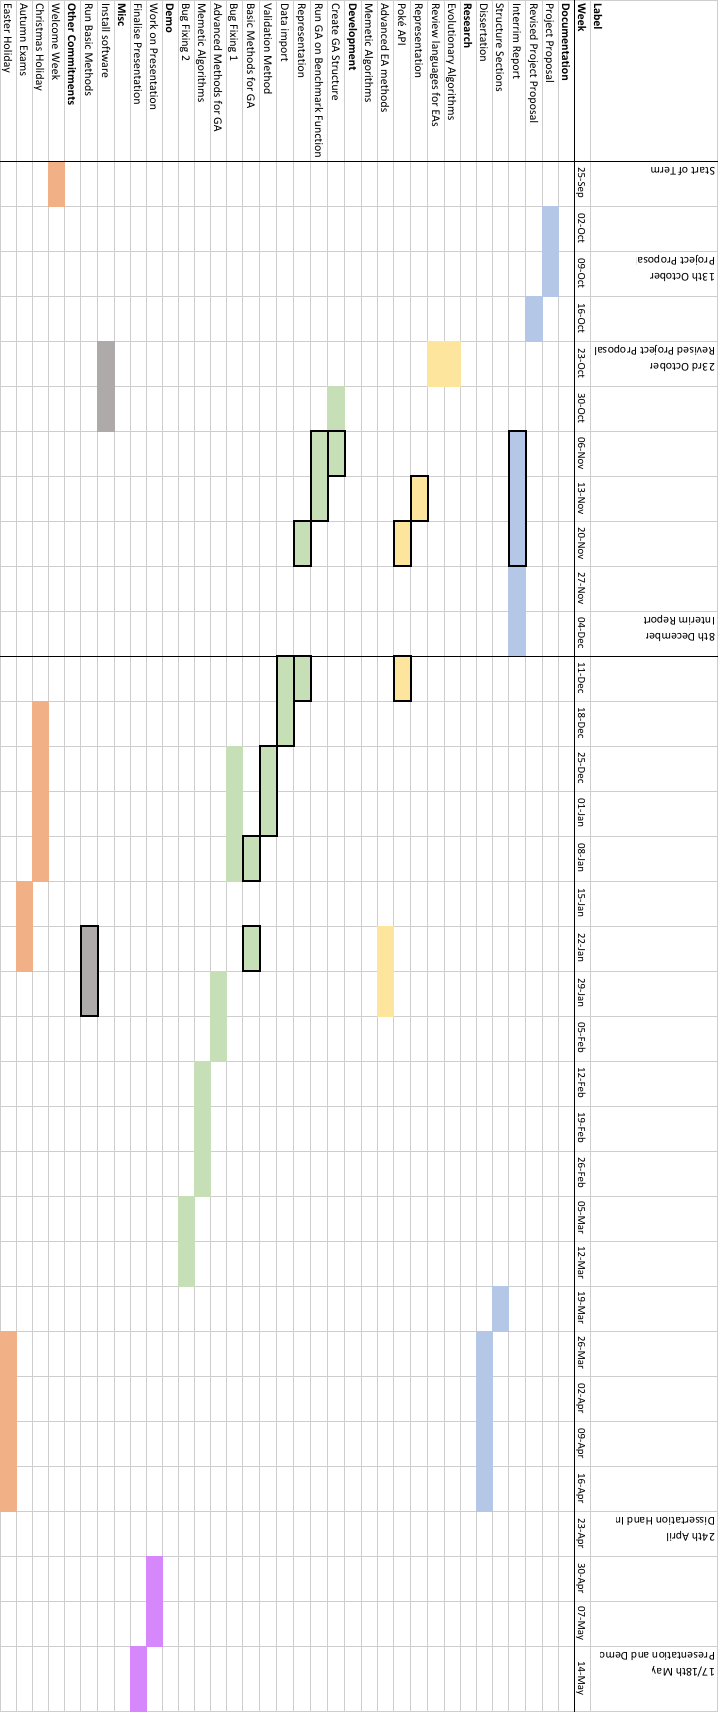
\includegraphics[height=24.8cm]{workPlan.png}
\end{center}


%Bibliography
\subsection{References}
\bibliography{Dissertation}
\bibliographystyle{plain}


\end{document}
